% Figura cuerpo B2 (3.1.2): por qué no conviene rebajar el precio: el coste por unidad efectiva
\documentclass[tikz,border=3pt]{standalone}
\usepackage[T1]{fontenc}
\usepackage[utf8]{inputenc}
\usepackage{amsmath}
\usetikzlibrary{arrows.meta,calc,positioning}
\begin{document}
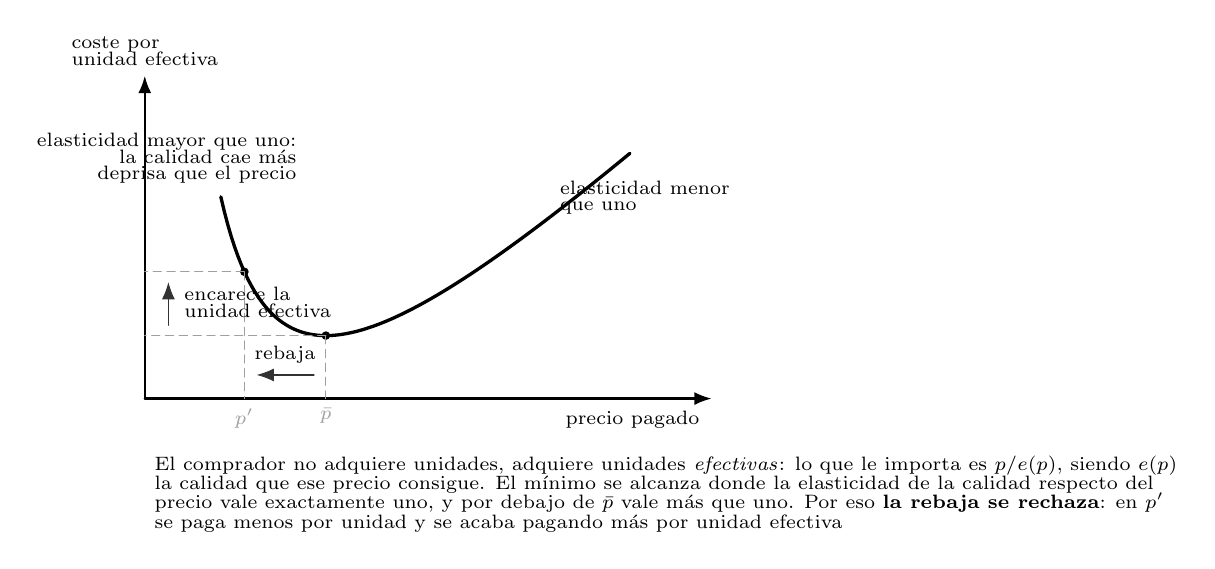
\begin{tikzpicture}[>={Latex[length=2.2mm]}, line cap=round, font=\footnotesize,
  eje/.style={->, thick},
  curva/.style={very thick},
  guia/.style={densely dashed, gray!75},
  pto/.style={circle, fill=black, inner sep=1.1pt}]

  \draw[eje] (0,0) -- (7.2,0) node[below left=1pt, font=\scriptsize]{precio pagado};
  \draw[eje] (0,0) -- (0,4.1) node[above, font=\scriptsize, align=left]{coste por\\[-2pt]unidad efectiva};

  \draw[curva] plot[domain=0.42:2.68, samples=120] ({2.3*\x},{2.2*(\x+1/\x)-3.6});

  % Mínimo y punto rebajado
  \node[pto] (M) at (2.30,0.80) {};
  \node[pto] (R) at (1.265,1.61) {};
  \draw[guia] (2.30,0.80) -- (2.30,0) node[below, font=\scriptsize]{$\bar{p}$};
  \draw[guia] (2.30,0.80) -- (0,0.80);
  \draw[guia] (1.265,1.61) -- (1.265,0) node[below, font=\scriptsize]{$p'$};
  \draw[guia] (1.265,1.61) -- (0,1.61);

  % Las dos flechas del razonamiento
  \draw[->, gray!40!black, shorten >=2pt, shorten <=2pt] (2.22,0.30) -- (1.35,0.30);
  \node[anchor=south, font=\scriptsize] at (1.78,0.32) {rebaja};
  \draw[->, gray!40!black, shorten >=2pt, shorten <=2pt] (0.30,0.86) -- (0.30,1.55);
  \node[anchor=west, font=\scriptsize, align=left] at (0.38,1.22) {encarece la\\[-2pt]unidad efectiva};

  \node[anchor=east, font=\scriptsize, align=right] at (2.05,3.05)
    {elasticidad mayor que uno:\\[-2pt]la calidad cae más\\[-2pt]deprisa que el precio};
  \node[anchor=west, font=\scriptsize, align=left] at (5.15,2.55)
    {elasticidad menor\\[-2pt]que uno};

  \node[align=left, anchor=north west, font=\scriptsize] at (0,-0.60)
    {El comprador no adquiere unidades, adquiere unidades \textit{efectivas}: lo que le importa es $p/e(p)$, siendo $e(p)$\\[-1pt]la calidad que ese precio consigue. El mínimo se alcanza donde la elasticidad de la calidad respecto del\\[-1pt]precio vale exactamente uno, y por debajo de $\bar{p}$ vale más que uno. Por eso \textbf{la rebaja se rechaza}: en $p'$\\[-1pt]se paga menos por unidad y se acaba pagando más por unidad efectiva};
\end{tikzpicture}
\end{document}
